%%%%%%%%%%%%%%%%%%%%%%%%%%%%%%%%%%%%%%%%%%%%%%%%%%%%%%%%%%%%%%%%%%%%
%% I, the copyright holder of this work, release this work into the
%% public domain. This applies worldwide. In some countries this may
%% not be legally possible; if so: I grant anyone the right to use
%% this work for any purpose, without any conditions, unless such
%% conditions are required by law.
%%%%%%%%%%%%%%%%%%%%%%%%%%%%%%%%%%%%%%%%%%%%%%%%%%%%%%%%%%%%%%%%%%%%

\documentclass[
  digital, %% This option enables the default options for the
           %% digital version of a document. Replace with `printed`
           %% to enable the default options for the printed version
           %% of a document.
  table,   %% Causes the coloring of tables. Replace with `notable`
           %% to restore plain tables.
  lof,     %% Prints the List of Figures. Replace with `nolof` to
           %% hide the List of Figures.
  lot,     %% Prints the List of Tables. Replace with `nolot` to
           %% hide the List of Tables.
  %% More options are listed in the user guide at
  %% <http://mirrors.ctan.org/macros/latex/contrib/fithesis/guide/mu/fi.pdf>.
]{fithesis3}
%% The following section sets up the locales used in the thesis.
\usepackage[resetfonts]{cmap} %% We need to load the T2A font encoding
\usepackage[T1,T2A]{fontenc}  %% to use the Cyrillic fonts with Russian texts.
\usepackage[slovak]{babel}        %% foreign texts to be typeset as follows:

%%
%% The following section sets up the metadata of the thesis.
\thesissetup{
    date          = \the\year/\the\month/\the\day,
    university    = mu,
    faculty       = fi,
    type          = bc,
    author        = Martin Styk,
    gender        = m,
    advisor       = {Ing. Mgr. et Mgr. Zdeněk Říha, Ph.D.},
    title         = {Analýza inštalačných APK súborov pre OS Android},
    keywords      = {APK súbor, Android, Apktool, malvér, analýza aplikácií, AndroidManifest.xml},
}
\thesislong{abstract}{
    Práca sa zaoberá získavaním metadát o inštalačných APK súboroch pre mobilný operačný systém Android. V rámci práce je vytvorená rozsiahla databáza APK balíčkov. Na základe analýzy týchto súborov sú určené štatistické vlastnosti APK súborov a príslušných aplikácií. Ako súčasť tejto práce je implementovaný nástroj na hromadné sťahovanie APK súborov, ich analýzu a výpočet štatistických dát nad množinou APK súborov. Práca sa zaoberá aj bezpečnosťou aplikácií a detekciou modifikovaných APK súborov. V práci je navrhnutá metóda detekcie upravených a prebalených APK balíčkov, ktorá je aj prakticky implementovaná. 
    V teoretickej časti je popísaná štruktúra APK balíčkov a súborov v nich obsiahnutych. 
}
\thesislong{thanks}{
    Rád by som sa poďakoval vedúcemu práce Ing. Mgr. et Mgr. Zdeňkovi Říhovi, Ph.D. za venovaný čas, ochotu a cenné pripomienky, ktoré mi pomohli pri tvorbe tejto práce.
}
%%XML
\usepackage{listings}

\usepackage{color}
\definecolor{gray}{rgb}{0.4,0.4,0.4}
\definecolor{light-gray}{rgb}{0,0,0}
\definecolor{darkblue}{rgb}{0.0,0.0,0.6}
\definecolor{cyan}{rgb}{0.0,0.6,0.6}


\lstset{
  basicstyle=\ttfamily,
  columns=fullflexible,
  showstringspaces=false,
  captionpos=b,
}

\lstdefinelanguage{XML}
{
  morestring=[b]",
  morestring=[s]{>}{<},
  morecomment=[s]{<?}{?>},
  stringstyle=\color{black},
  identifierstyle=\color{darkblue},
  keywordstyle=\color{cyan},
  morekeywords={xmlns,version,type}% list your attributes here
}
\renewcommand{\lstlistingname}{Kód}

%% The following section sets up the bibliography.
\usepackage{csquotes}
\usepackage[              %% When typesetting the bibliography, the
  backend=biber,          %% `numeric` style will be used for the
  style=iso-numeric,          %% entries and the `numeric-comp` style
  citestyle=numeric-comp, %% for the references to the entries. The
  sorting=none,           %% entries will be sorted in cite order.
  sortlocale=auto,        %% For more unformation about the available
]{biblatex}               %% `style`s and `citestyles`, see:
%% <http://mirrors.ctan.org/macros/latex/contrib/biblatex/doc/biblatex.pdf>.
\addbibresource{bibliografie.bib} %% The bibliograpic database within
                          %% the file `example.bib` will be used.
\usepackage{makeidx}      %% The `makeidx` package contains
\makeindex                %% helper commands for index typesetting.
%% These additional packages are used within the document:
\usepackage{paralist}
\usepackage{amsmath}
\usepackage{amsthm}
\usepackage{amsfonts}
\usepackage{url}
\usepackage{menukeys}
\usepackage{fancybox}
\usepackage{pgf-pie}
\usepackage{tikz}
\usepackage{longtable}
\usepackage{tabularx}

\newcommand{\zv}{\textit}
\newcommand{\cesta}{\zv}

\begin{document}
\chapter{Úvod}
\zv{TBD}


%% Operačný systém Android 
%\chapter{Operačný systém Android}
Android je mobilný operačný systém navrhnutý primárne pre zariadenia s~dotykovou obrazovkou. Android je dominantným operačným systémom na trhu s~mobilnými zariadeniami ako sú chytré telefóny a tablety. V~treťom kvartáli roku 2015 dosahoval až 84,7\% podiel na trhu operačných systémov pre mobilné zariadenia~\cite{Westenberg2015}. Systém je založený na linuxovom jadre.

Android je aktuálne vyvíjaný spoločnosťou Google ako open source projekt. Existuje aktívna komunita vývojárov podieľajúca sa na vývoji projektu Android Open Source Project. Väčšina Android zariadení sa predáva s~kombináciou open source a proprietárneho softvéru. Medzi proprietárne časti zdrojového kódu patria nadstavby výrobcov telefónov a služby spoločnosti Google, tzv. Google services. Android nemá žiadny centralizovaný systém aktualizácií. To má za následok, že veľká časť zariadení nedostáva aktualizácie dostatočne často. Až 87,7\,\% zariadení obsahuje kritické bezpečnostné zraniteľnosti, ktoré sú známe, ale nie sú opravené kvôli slabej podpore~\cite{Thomas2015}.


\section{História}
Začiatok vývoja operačného systému, ktorý je dnes známy ako Android siaha do roku 2003, kedy vznikla spoločnosť Android, Inc. Prvotným zámerom spoločnosti bola tvorba systému pre digitálne fotoaparáty, avšak kvôli malému trhu bol vývoj preorientovaný na operačný systém pre mobilné zariadenia. Zakladatelia spoločnosti Andy Rubin, Rich Miner, Nick Sears  a Chris White plánovali vývoj operačného systému pre chytré mobilné zariadenia, ktoré dokážu efektívne využívať prostredie a preferencie užívateľov~\cite{Beavis2008}. Spoločnosť Android bola v~roku 2005 kúpená spoločnosťou Google za približne 50 miliónov dolárov~\cite{Rosoff2011}. 5.\,novembra 2007 bolo predstavené konzorcium \zv{Open Handset Alliance}, skladajúce sa z~výrobcov mobilných zariadení, mobilných operátorov a výrobcov komponentov pre mobilné zariadenia. Hlavným cieľom konzorcia je vývoj otvorených mobilných štandardov~\cite{OHA}. Prvým predstaveným produktom tejto skupiny bol operačný systém založený na linuxovom jadre -- Android. Prvým komerčne dostupným chytrým telefónom s~operačným systémom Android sa 22.\,novembra 2008 stal \zv{HTC Dream}. Od roku 2008 sa systém inkrementálne vylepšuje a vyvíja. Bolo vydaných množstvo opráv, vylepšení a nových funkcií. Začínajúc od verzie \zv{Android 1.5 Cupcake}, je každá verzia pomenovaná podľa cukroviniek.

\section{Architektúra systému}
Operačný systém Android je možné dekomponovať do piatich sekcií a štyroch základných architektonických vrstiev organizovaných v~zásobníkovej štruktúre~\cite{Gunasekera2012} zobrazenej na obrázku \ref{fig:struktura}.
\begin{figure} [htb]
 \centering
	\ovalbox{
		\begin{minipage}[b]{10cm}	
			\begin{center}
			Aplikácie
			\end{center}					
		\end{minipage}
		}\\
	\ovalbox{
		\begin{minipage}[b]{10cm}	
			\begin{center}
			Aplikačný rámec
			\end{center}					
		\end{minipage}
		}\\
	\ovalbox{
		\begin{minipage}[b]{10cm}	
			\begin{center}
			Knižnice \hfill Android Runtime (DVM)
			\end{center}
		\end{minipage}
		}\\
	\ovalbox{
		\begin{minipage}[b]{10cm}	
			\begin{center}
			Linuxové jadro
			\end{center}					
		\end{minipage}
		}	
  \caption{Vrstevnatá architektúra systému Android}
  \label{fig:struktura}
\end{figure}
\subsection{Linuxové jadro}
Najnižšiu vrstvu predstavuje Linux jadro vo verzií 2.6. Jadro je upravené za účelom optimalizácie spotreby energie a operačnej pamäte, podporuje preemptívny multitasking. Táto vrstva poskytuje abstrakciu medzi hardvérom zariadenia a vyššími softvérovými vrstvami~\cite{Allen2010}. Na tejto vrstve sa nachádzajú ovládače hardvérových komponent ako fotoaparát, dotyková obrazovka alebo sieťové rozhranie~\cite{architecture}.
\subsection{Android Runtime a Dalvik Virtual Machine}
\zv{Dalvik Virtual Machine} je virtuálny stroj slúžiaci na exekúciu Android aplikácií~\cite{dalvik}. Je obdobou virtuálneho stroja \zv{JVM (Java Virtual Machine)} používaného pri jazyku Java. Virtuálny stroj \zv{Dalvik} využíva nízkoúrovňovú funkcionalitu linuxového jadra. Každá aplikácia je spustená vo vlastnom procese a na vlastnej inštancii virtuálneho stroja. Tento prístup zaručuje, že aplikácie sa navzájom neúmyselne neovplyvňujú, nepristupujú priamo k~hardvéru zariadenia a využívajú abstrakciu, ktorá zabezpečuje ich platformovú nezávislosť~\cite{architecture}.  Od verzie Android 5.0 je virtuálny stroj \zv{Dalvik} plne nahradený novým behovým prostredím \zv{Android Runtime} (\zv{ART}).
\subsection{Knižnice}
Android obsahuje množstvo knižníc využívaných vývojármi alebo samotným systémom. Špecifickou skupinou sú natívne knižnice jadra, často označované ako \zv{Dalvik knižnice}, ktoré obsahujú kód pre interakciu s~inštanciou virtuálneho stroja, ale aj napríklad knižnice pre prístup k~systému súborov. Veľká časť knižníc obsiahnutá v~tejto vrstve využíva natívny kód v~jazyku C/C++. Takéto knižnice slúžia ako obal okolo C/C++ kódu, ku ktorému  sprostredkúvajú prístup pomocou jazyka Java. Táto vrstva obsahuje niektoré štandardné knižnice známe z~jazyka Java, ktoré sú upravené pre využitie na operačnom systéme Android, ale aj knižnice špecifické pre platformu Android, tzv. \zv{Android knižnice}~\cite{Hashimi2009}.
\subsection{Aplikačný rámec}
Vrstva aplikačného rámca poskytuje vysokoúrovňové služby používané na manažment aplikácie. Využíva koncept Android aplikácií, ktoré sa skladajú z~viacerých komponent. Kľúčové služby poskytované aplikačným rámcom sú~\cite{architecture}: 
\begin{itemize}
	\item \bod{Activity Manager}  --  ovláda životný cyklus aktivít a spravuje zásobník naposledy spustených aktivít,
	\item \bod{Content Provider}  --  umožňuje zdieľanie dát medzi aplikáciami,
	\item \bod{Resource Manager}  --  poskytuje prístup k~zdrojovým súborom ako reťazce, obrázky, dizajny obrazoviek,
	\item \bod{Notification Manager}  --  umožňuje aplikácii zobrazovať upozornenia,
	\item \bod{View system}  --  poskytuje prvky grafického používateľského rozhrania aplikácie,
	\item \bod{Package Manager}  --  umožňuje aplikáciám získať informácie o~ostatných aplikáciách nainštalovaných na zariadení,
	\item \bod{Telephony Manager}  --  umožňuje aplikáciám získať informácie o~stave telefónnych služieb,
	\item \bod{Location Manager}  --  poskytuje aplikáciám informácie o~polohe zariadenia.
\end{itemize}
\subsection{Vrstva aplikácií}
Na vrchole vrstevnatej architektúry systému Android sú aplikácie, ktoré využívajú súčinnosť všetkých spomenutých vrstiev. 

\section{Aplikácie}
\subsection{Distribúcia aplikácií}

APK súbory predstavujúce inštalačné balíčky Android aplikácií sú najčastejšie distribuované pomocou obchodu s~aplikáciami. Oficiálny obchod pre Android zariadenia je \zv{Google Play}. Aplikácie môžu byť distribuované pomocou alternatívnych obchodov ako napríklad \zv{Amazon Appstore} alebo \zv{SlideMe}. Operačný systém Android v~základnom nastavení neumožňuje inštaláciu aplikácií z~iných zdrojov ako \zv{Google Play}. Inštalácia z~neznámych zdrojov môže byť povolená v~nastaveniach zariadenia. Inštalačné APK balíčky je možné získať aj zo stránok na zdieľanie ľubovoľného obsahu, na ktorých sa často distribuujú aplikácie ktoré sú v~oficiálnych zdrojoch platené. Takéto súbory sú často modifikované a môžu obsahovať potenciálny škodlivý kód. Často ich označujeme ako prebalené aplikácie. Viac informácií o~prebalených aplikáciách sa nachádza v~kapitole \ref{Repackaged}.

\subsection{Inštalácia aplikácií}
Aplikácie môžeme rozdeliť na dve skupiny:
\begin{itemize}
\item Predinštalované aplikácie – často označované aj ako systémové aplikácie. Tieto aplikácie sú nainštalované spolu so systémom a často nemôžu byť bežným používateľom odinštalované. Príkladom je základná aplikácia pre fotoaparát, kontakty alebo telefón.
\item Aplikácie nainštalované používateľom – Aplikácie nainštalované jedným z~nasledujúcich spôsobov~\cite{Elenkov2015}:
\begin{itemize}
\item prostredníctvom obchodu s~aplikáciami, najčastejšie \zv{Google Play Store},
\item prostredníctvom nástroja \zv{Android Debug Bridge} (\zv{ADB}) ktorý je obsiahnutý, v~\zv{Android SDK} a umožňuje inštaláciu a ladenie aplikácií na zariadení pripojenom k~počítaču pomocou USB kábla
\item otvorením APK balíčka umiestneného v~zariadení.
\end{itemize}
\end{itemize}

\noindent Základnou aplikáciou starajúcou sa o~inštaláciu APK balíčkov je \zv{PackageInstaller}, ktorý poskytuje užívateľské rozhranie na komunikáciu so službou \zv{PackageManager}. \zv{PackageManager}  poskytuje v~rámci triedy \zv{PackageManagerService.java} API pre inštaláciu, aktualizáciu a odinštaláciu aplikácií. Natívny démon \zv{installd} prijíma požiadavky od služby \zv{PackageManagerService.java} s~ktorou komunikuje prostredníctvom lokálneho soketu \cesta{/dev/socket/installed}. Služba \zv{PackageManager} a démon \zv{installd} sú spustené pri štarte systému. \zv{PackageManager} čaká na pridanie požiadavky na inštaláciu do zoznamu inštalovaných aplikácií. Pri inštalácii analyzuje súbor \zv{AndroidManifest.xml} a relevantné informácie ukladá do súborov \cesta{/data/system/packages.xml} a \cesta{/data/system/packages.list}. Priečinok, do ktorého sa APK súbor rozbalí, vytvára démon \zv{installd}, o~rozbalenie a kopírovanie obsahu sa stará \zv{PackageManager}. Predinštalované (systémové) aplikácie sú inštalované do zložky \cesta{/system/app/}, aplikácie inštalované užívateľom do zložky \cesta{/data/app/}. Súbor \zv{classes.dex}, ktorý je obsiahnutý v~APK balíčku je kopírovaný do \cesta{/data/dalvik-cache/}. \zv{PackageManager} vytvorí priečinok \cesta{/data/data/nazov\_balíčku} v~ktorom sa nachádzajú preferencie, databázy alebo natívne knižnice aplikácie~\cite{Parmar2013}.

%% Apk súbory
%\chapter{APK súbory}
\label{APKsubory}
APK súbory sú balíčky používané operačným systémom Android. Celý názov ukrytý za skratkou APK je Android application package file. Tieto súbory slúžia na distribúciu aplikácií v operačnom systéme Android. Ich použitie a význam je analogický ako pri MSI\footnote{\url{Windows Installer Package https://technet.microsoft.com/en-us/library/cc978328.aspx}} balíčkoch používaných v systéme Microsoft Windows, alebo DEB\footnote{\url{https://www.debian.org/doc/manuals/debian-faq/ch-pkg\_basics.en.html}} balíčkoch používaných v niektorých linuxových distribúciách. APK súbory sú asociované s príponou .apk a príslušný MIME typom \zv{application/vnd.android.package-archive}.

Štruktúra APK balíčkov vychádza z JAR\footnote{Java archive} balíčkov -- súborov používaných na distribúciu aplikácií alebo knižníc na platforme Java. Formát APK rozširuje všeobecnejší JAR formát o súbory, ktoré sú špecifické pre cieľovú platformu, ktorou je operačný systém Android. Zároveň si však ponecháva vlastnosti JAR súborov. APK balíčky sú archívne súbory v ZIP\footnote{\url{https://en.wikipedia.org/wiki/Zip\_(file_format)}} formáte.  Keďže APK používajú ZIP formát, k ich obsahu môžeme jednoducho pristúpiť rozbalením archívu štandardným spôsobom.  APK súbory vznikajú ako výstup kompletnej kompilácie a zabalenia aplikácií pre Android. APK súbor každej aplikácie obsahuje všetky potrebné súbory na jej inštaláciu a spustenie. Medzi týmito súbormi sa typicky nachádza \zv{classes.dex} súbor obsahujúci skompilovaný zdrojový kód, \zv{resources.arsc} súbor ktorý obsahuje skompilované zdroje aplikácie, súbor \zv{AndroidManifest.xml} a neskompilované súbory ako sú napríklad obrázky.\\\\
\begin{figure}[htb]
  \begin{center}
    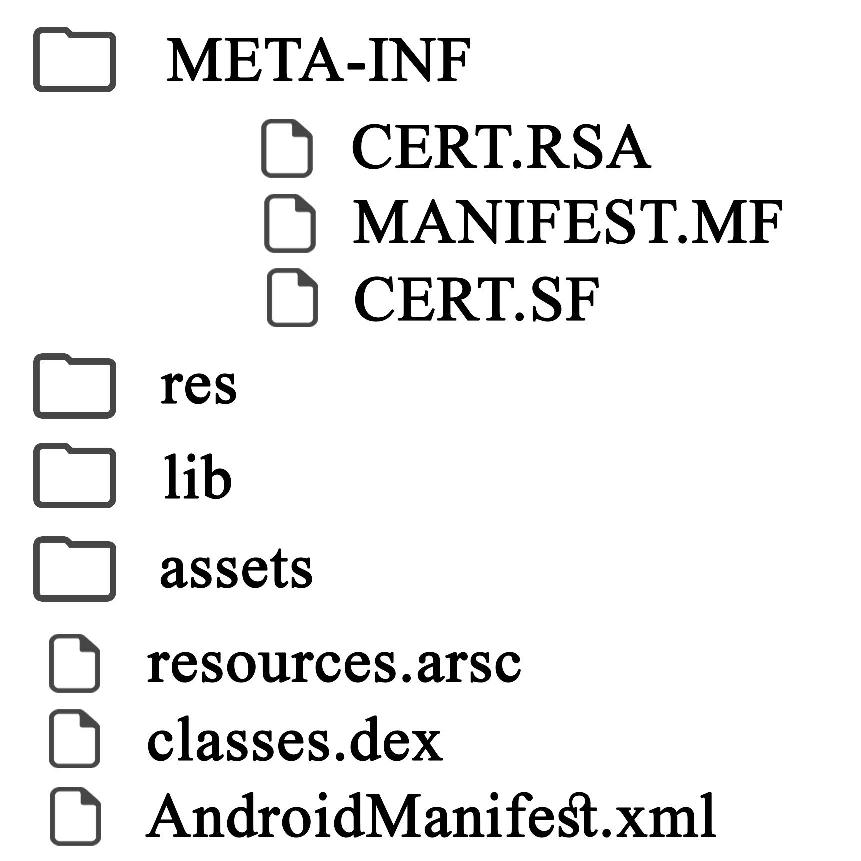
\includegraphics[width=60mm]{images/apkStructure.pdf}
  \end{center}
  \caption{Typická štruktúra APK súboru}
\end{figure}

\section{Priečinok META-INF}
\label{META-INF}
Priečinok obsahujúci súbory, ktorých úlohou je zaručiť integritu ostatných súborov v APK balíčku a s ňou spojenú bezpečnosť celého systému. V prípade detekcie pozmenených súborov a narušenia integrity operačný systém Android nedovolí inštaláciu APK balíčku. Po každej zmene je nutné balíček digitálne podpísať.


\subsection*{CERT.RSA}
\label{CERT.RSA} 
Súbor obsahujúci verejný kľúč ktorý slúži na overenie digitálneho podpisu balíčka.
\subsection*{MANIFEST.MF}
\label{MANIFEST.MF}
Súbor obsahujúci relatívne cesty a SHA-1 hashe \footnote{reťazce v Base64 kódovaní} všetkých súborov v APK balíčku. Tento súbor neobsahujú len APK súbory, je typický pre každý JAR archív.\\\\
Typický začiatok súboru \zv{MANIFEST.MF} vyzerá nasledovne: \\

\begin{verbatim}
Manifest-Version: 1.0
Built-By: 0.12.2
Created-By: Android Gradle 0.12.2

Name: res/drawable-xhdpi-v4/libraries.png
SHA1-Digest: VvgaO1jpW3iS1nBBikD/urdbN58=

Name: res/layout/activity_settings.xml
SHA1-Digest: 1coP1lt9Lmccc7SMZGHxNv4bbKs=
\end{verbatim}

\subsection*{CERT.SF}
\label{CERT.SF}
Súbor podobný ako \zv{MANIFEST.MF}, avšak namiesto SHA-1 hashov samotných súborov obsahuje SHA-1 hashe záznamov o týchto súboroch z \zv{MANIFEST.MF}. Okrem toho obsahuje aj hash celého súboru \zv{MANIFEST.MF}. \newline Záznam o jednom súbore v APK balíčku v súbore \zv{CERT.SF} vyzerá nasledovne: \newline
\begin{verbatim}
Name: res/drawable-xhdpi-v4/libraries.png
SHA1-Digest: Slg56lqothjvmaBikD/urdb7q6=
\end{verbatim}\mbox{}\\
Reťazec \zv{Slg56lqothjvmaBikD/urdb7q6=} reprezentuje SHA-1 hash nasledujúceho záznamu zo súboru \zv{MANIFEST.MF}:\mbox{}\\
\begin{verbatim}
“Name: res/drawable-xhdpi-v4/libraries.png
SHA1-Digest: VvgaO1jpW3iS1nBBikD/urdbN58=
”\end{verbatim}

\section{Priečinok res}
\label{res}
Priečinok obsahujúci zdrojové súbory ako napríklad obrázky, zvuky alebo ikony. Okrem multimediálnych súborov obsahuje taktiež zdrojové XML súbory určujúce vzhľad obrazoviek, použité grafické štýly, alebo texty použité v aplikácii. Niektoré z týchto XML súborov môžu byť skompilované do binárneho formátu. V zdrojovom kóde sú tieto zdroje odkazované pomocou unikátnych identifikátorov. Identifikátory sú generované počas kompilácie nástrojom aapt a nachádzajú sa v projektovej triede \zv{R}. Pre každý typ zdrojového súboru je generovaná podtrieda triedy \zv{R}. Všetky zdroje aplikácie by mali byť externalizované a uložené v špecifickom podpriečinku v tomto adresári. \\\\
\textbf{Podporované podpriečinky}
\begin{itemize}
\item animator - obsahuje XML súbory definujúce property animácie\cite{article-full}
\item anim - obsahuje XML súbory definujúce tween animácie, môže obsahovať aj property animácie
\item color - obsahuje XML súbory definujúce farby a ich zmeny na základe stavu objektov na ktoré sú aplikované
\item drawable - obsahuje obrázky vo formáte PNG, 9.PNG, JPG, GIF alebo XML súbory skompilované do formy vykresliteľných obrázkov
\item mipmap - ikony aplikácie s rôznou hustotou pixelov
\item layout - obsahuje súbory vo formáte XML definujúce vzhľad rozmiestnenie prvkov na obrazovke
\item menu - obsahuje súbory XML definujúce menu aplikácie
\item raw - obsahuje súbory ktoré musia byť uložené a použité v neskomprimovanej forme a kvalite
\item values - obsahuje súbory vo formáte XML definujúce hodnoty textových reťazcov, farieb, štýlov, základných rozmerov
\item xml - obsahuje XML súbory, ktoré môžu byť načítané počas behu aplikácie
\end{itemize}

\noindent V spomenutých priečinkoch sú uložené základné zdroje aplikácie. Tieto zdrojové súbory určujú základný dizajn a obsah aplikácie. Avšak rôzne typy Android zariadení môžu využívať rôzne zdrojové súbory. Alternatívne zdroje sa využívajú na prispôsobenie dizajnu a obsahu veľkosti a aktuálnej konfigurácií zariadenia. Sú umiestnené v priečinku, ktorého názov pozostáva z typu zdrojového súboru, ktorý korešponduje so základným názvom priečinku a názvu hodnoty konfiguračného atribútu pre ktorý je tento priečinok určený. Je možné kombinovať viacero konfiguračných atribútov.\\\\
\textbf{Najpoužívanejšie atribúty}
\begin{itemize}
\item Jazyk a región – jazyk je definovaný podľa ISO 639-1\footnote{http://www.iso.org/iso/home/standards/language\_codes.htm} kódovania s možnosťou rozšírenia pomocou ISO 3166-1-alpha-2 regionálneho kódu. Napríklad obrázky špecifické pre zariadenia s francúzskym jazykom sa nachádzajú v priečinku \cesta{res/drawable-fr}
\item Veľkosť obrazovky –  v závislosti na veľkosti a rozlíšení obrazovky rozlišuje štyri možné hodnoty -- small, normal, large, xlarge
\item Orientácia obrazovky – v závislosti na orientácii zariadenia hodnota port pre zariadenie vo vertikálnej polohe, hodnota land pre polohu horizontálnu
\item Hustota obrázkových bodov obrazovky -  hodnoty určujúce vhodnosť zdrojových súborov vzhľadom na hustotu obrázkových bodov obrazovky daného zariadenia
\end{itemize}


\section{Priečinok lib}
\label{lib}
Priečinok obsahujúci skompilovaný zdrojový kód natívnych knižníc. Tieto knižnice sú špecifické pre typ procesora. V závislosti na architektúre procesora obsahuje podpriečinky : \zv{armeabi, armeabi-v7a, arm64-v8a, x86, x86\_64, mips}.

\section{Priečinok assets}
\label{assets}
Priečinok obsahujúci súbory uložené a používané v originálnej neskomprimovanej forme. V tomto priečinku sa často nachádzajú textové súbory, html súbory, licenčné informácie, obrázky alebo textúry. Na rozdiel od priečinku \cesta{res/raw/}, zdrojovým súborom v umiestneným v priečinku assets nie sú pridelené unikátne identifikátory uložené v triede \zv{R.java}. K súborom sa pristupuje ako k dátam uloženým v bežnom súborovom systéme. Trieda \zv{AssetManager} poskytuje funkcionalitu na čítanie súborov ako prúdu bytov a  navigovanie v tomto priečinku.

\section{resources.arsc}
\label{resources.arsc}
Súbor obsahujúci mapovanie medzi zdrojovými súbormi  z priečinku \zv{res} a ich identifikátormi.  Vytvára sa počas kompilácie. Obsahuje XML súbory v binárnom formáte.

\section{classes.dex}
\label{classes.dex}
\zv{Classes.dex} je súbor obsahujúci skompilovaný zdrojový kód aplikácie.  Zdrojové súbory Android aplikácií sú napísané v jazyku Java. Java súbory sú skompilované do Java bytekódu pomocou bežného kompilátoru pre platformu Java. Výsledkom tejto kompilácie sú súbory s príponou \zv{class}, ktoré sú následne preložené do Dalvik bytekódu pomocou nástroja \zv{dx} ktorý je súčasťou Android Software Developement Kit. Výstupom nástroju \zv{dx} je jediný súbor obsahujúci skompilovaný celý výkonný zdrojový kód aplikácie -- \zv{classes.dex}. Tento súbor je skomprimovanou a optimalizovanou verziou všetkých \zv{class} súborov. Takto skompilovaný program môže byť vykonaný len vo virtuálnom stroji Dalvik, alebo v novšom prostredí ART (Android Runtime) používanom primárne od verzie Android 5.0 „Lollipop“.

\section{AndroidManifest.xml} 
\label{AndroidManifest.xml}
http://developer.android.com/guide/topics/manifest/manifest-intro.html
Súbor ktorý musí obsahovať každá Android aplikácia. Tento súbor poskytuje informácie o aplikácii operačnému systému Android. Neobsahuje žiadny výkonný kód. Definuje meno a verziu, ktoré slúžia ako unikátny identifikátor danej aplikácie. Popisuje všetky komponenty z ktorých sa aplikácia skladá, cesty k použitým knižniciam, minimálny vyžadovaný level Android API, oprávnenie vyžadované aplikáciu na prístup k chráneným častiam Android API a taktiež oprávnenia, ktoré sú vyžadované od iných komponent pri pokuse komunikovať s danou aplikáciou. Súbor \zv{AndroidManifest.xml}, ktorý nájdeme v APK balíčku je vo formáte binárneho XML súboru. Je ho však možné previesť do klasického čitateľného XML formátu.

Keďže \zv{AndroidManifest.xml} je základným súborom poskytujúcim metadáta o Android aplikácii a APK súbore, informácie získané z tohto súboru tvoria veľkú časť štatistických dát zbieraných a vyhodnocovaných v tejto práci. Preto sa detailnejšie pozrieme na jeho štruktúru a niektoré dôležité elementy, ktoré obsahuje.\\ Nasledujúci diagram ukazuje základnú štruktúru tohto XML súboru.
\begin{lstlisting} [language=XML, caption= {Základná štruktúra súboru AndroidManifest.xml}]
<?xml version="1.0" encoding="utf-8"?>
<manifest>
    <uses-permission />
    <permission />
    <uses-sdk />
    <uses-configuration />  
    <uses-feature />  
    <supports-screens />  
    <compatible-screens />  
    <application>
        <activity />
        <service/>
        <receiver/>
        <provider/>
        <uses-library />
    </application>
</manifest>
\end{lstlisting}

\subsection{Element manifest}
\lstset{language=XML}
\begin{lstlisting}
<manifest xmlns:android="URL"
          package="string"
          android:sharedUserId="string"
          android:sharedUserLabel="string resource"
          android:versionCode="integer"
          android:versionName="string"
          android:installLocation=["auto" | "internalOnly" |
                                        "preferExternal"] >
</manifest>
\end{lstlisting}
\zv{AndroidManifest.xml} obsahuje element manifest ako koreňový prvok. Tento element je povinný a každý manifest ho obsahuje práve jeden. \newline\newline
\noindent Element manifest definuje atribúty:\\
\begin{itemize}
\item xmlns:android – povinný atribút definujúci menný priestor
\item package – meno balíku aplikácie, povinný atribút definujúci identitu aplikácie. Meno balúku nemôže byť zmenené
\item android:sharedUserId – identifikátor aplikácie zdieľaný s ostatnými aplikáciami za účelom vzájomnej komunikácie
\item android:sharedUserLabel – čitateľná podoba android:sharedUserId identifikátoru
\item android:versionCode – interná informácia o verzii aplikácie. Tento atribút je využívaný len na rozoznanie novších verzíí od starších. Novšie aplikácie obsahujú vyššiu hodnotu
\item android:versionName – informácia o verzií aplikácie prezentovaná užívateľom. Pre systém Android neposkytuje informáciu o verzií aplikácie, tú obsahuje atribút android:versionCode.
\item android:installLocation – určuje miesto základné miesto inštalácie aplikácie. Pokiaľ je aplikáciu možné nainštalovať len do vnútornej pamäti zariadenia, obsahuje hodnotu internalOnly. Takáto aplikácia nemôže byť presunutá na externé pamäťové médium (typicky SD karta). Táto hodnota je základnou použitou možnosťou, ak tento atribút nie je definovaný. V prípade hodnoty auto sú aplikácie inštalované vo vnútornej pamäti, ale môžu byť presunuté do pamäti externej. Hodnota preferExternal zabezpečí, že systém sa pokúsi o inštaláciu na externé pamäťové médium. V prípade neúspechu sa použije interná pamäť
\end{itemize}

\subsection{Element uses-permission}
\lstset{language=XML}
\begin{lstlisting}
<uses-permission android:name="string"
        android:maxSdkVersion="integer" />
\end{lstlisting}
Prístup k niektorým dátam alebo častiam kódu je z dôvodu ochrany limitovaný. Android využíva princíp povolení\footnote{angl. permissions}. Povolenia môžu byť definované samotnou aplikáciou, inou aplikáciou alebo systémom Android. Aplikácia, ktorá chce pristupovať k chráneným dátam alebo používať chránené časti kódu, musí pomocou tagu uses-permissions deklarovať vyžadované povolenia. Prístupové povolenia sú aplikácii schválené užívateľom. Vo verzii Android 5.1 a starších, systém počas inštalácie oboznámi užívateľa so všetkými povoleniami, ktoré aplikácia vyžaduje. V prípade, že ich používateľ neschváli, aplikácia nebude nainštalovaná. Od verzie Android 6.0 užívateľ schvaľuje povolenia počas behu aplikácie.\\\\ 
Element uses-permission definuje atribúty:\\
\begin{itemize}
\item android:name – definuje názov povolenia
\item android:maxSdkVersion – najvyšší level Android API, pre ktorý je dané povolenie potrebné
\end{itemize}

\subsection{Element permission}
\lstset{language=XML}
\begin{lstlisting}
<permission android:description="string resource"
            android:icon="drawable resource"
            android:label="string resource"
            android:name="string"
            android:permissionGroup="string"
            android:protectionLevel=["normal"|"dangerous"| 
                                     "signature"|
                                     "signatureOrSystem"] />
\end{lstlisting}
Definuje bezpečnostné povolenie, ktoré môže byť použité na obmedzenie prístupu ku komponente aplikácie. Toto povolenie je následne používané aplikáciami, ktoré vyžadujú prístup k chránenej časti danej aplikácie.\\\\ Najdôležitejšie atribúty definované v rámci elementu permission:\\
\begin{itemize}
\item android:name – názov povolenia, aplikácie vyžadujúce dané povolenie uvádzajú túto hodnotu v atribúte android:name v tagu uses-permission. Názov musí byť unikátny a mal by dodržiavať konvencie pomenovávania jazyka Java.
\item android:permissionGroup – priradí toto povolenie do skupiny povolení (angl. Permission group). Táto skupina povolení musí byť deklarovaná v rámci elementu permission-group v niektorej z nainštalovaných aplikácií. Slúži na logické zoskupenie významovo podobných oprávnení.
\item android:protectionLevel – charakterizuje potenciálne riziko spojené s použitím daného povolenia. Táto hodnota určuje postup operačného systému pri rozhodovaní o udelení povolenia. 
Základnou hodnotou je „normal“, ktorá reprezentuje povolenia s nízkou mierou rizika. Tieto povolenia sú aplikácii automaticky schválené systémom Android počas inštalácie. Pre povolenia z zvýšenou mierou rizika je určená hodnota „dangerous“. Tieto povolenia typicky udeľujú aplikácií prístup k citlivým dátam alebo k prvkom Android zariadenia, ktoré môžu negatívne ovplyvniť jeho používanie. Pretože tento typ povolení prináša potenciálne riziko, systém ho nemôže udeliť automaticky, ale až po explicitnom súhlase používateľa.
V prípade, že tento atribút obsahuje hodnotu „signature“, povolenie je udelené automaticky a to len aplikáciám, ktorých certifikát je rovnaký ako certifikát aplikácie definujúcej dané povolenie.   
Hodnota „signatureOrSystem“ rozširuje hodnotu „signature“ a povolenia sú udelené aj aplikáciám Android system image.
\end{itemize}

\subsection{Element uses-sdk}
\lstset{language=XML}
\begin{lstlisting}
<uses-sdk android:minSdkVersion="integer"
          android:targetSdkVersion="integer"
          android:maxSdkVersion="integer" />
\end{lstlisting}
Element vyjadrujúci kompatibilitu aplikácie s verziou Androidu pomocou čísla verzie Android API.\\\\
Atribúty definované elementom uses-sdk:\\
\begin{itemize}
\item android:minSdkVersion – vyjadruje najnižší level API vyžadovaný aplikáciou. Pokiaľ je táto hodnota vyššia ako API úroveň zariadenia, systém zabráni inštalácií. Tento atribút by mala obsahovať každá aplikácia
\item android:targetSdkVersion – informuje o úrovni API na ktorej bola aplikácia testovaná a pre ktorú je primárne určená. V prípade, že zariadenie podporuje vyššiu verziu Android API ako definuje spomínaný atribút, aplikácia môže byť spustená v móde kompatibility s touto verziou API 
\item android:maxSdkVersion – najvyššia úroveň API kompatibilná s aplikáciou. Z dôvodu spätnej kompatibility nie je používanie tohto atribútu doporučené. Tento atribút bol využívaný len do verzie Android 2.0.1
\end{itemize}

\subsection{Element uses-feature}
\lstset{language=XML}
\begin{lstlisting}
<uses-feature
  android:name="string"
  android:required=["true" | "false"] />
\end{lstlisting}
Deklaruje hardvérovú alebo softvérovú vlastnosť \footnote{angl. feature} používanú aplikáciou. Tento element informuje externé entity o funkciách, ktoré aplikácia vyžaduje. Deklarované vlastnosti majú informačný charakter. Systém Android nekontroluje či zariadenie podporuje všetky vlastnosti deklarované aplikáciou. Tento element je využívaný službou Google Play na  filtrovanie aplikácií vyhovujúcich danému zariadeniu, a preto by mala byť deklarovaná každá vyžadovaná vlastnosť.\\\\ Element obsahuje nasledujúce atribúty:\\
\begin{itemize}
\item android:name – názov vyžadovanej vlastnosti
\item android:required – určuje, či aplikácia vyžaduje danú vlastnosť pre korektné fungovanie. Pokiaľ obsahuje hodnotu true, aplikácia nie je schopná korektne fungovať na zariadení nepodporujúcom danú vlastnosť
\end{itemize}

http://developer.android.com/guide/topics/manifest/uses-feature-element.html
\subsection{Element supports-screens}
\lstset{language=XML}
\begin{lstlisting}
<supports-screens android:resizeable=["true"| "false"]
                  android:smallScreens=["true" | "false"]
                  android:normalScreens=["true" | "false"]
                  android:largeScreens=["true" | "false"]
                  android:xlargeScreens=["true" | "false"]
                  android:anyDensity=["true" | "false"]
                  android:requiresSmallestWidthDp="integer"
                  android:compatibleWidthLimitDp="integer"
                  android:largestWidthLimitDp="integer"/>
\end{lstlisting}
Špecifikuje podporované typy obrazoviek. V prípade inštalácie na zariadení s väčšou obrazovkou ako aplikácia podporuje, informuje systém o potrebe využitia módu obrazovej kompatibility.\\\\ Väčšina atribútov deklaruje podporované veľkosti obrazoviek. Ďalšie atribúty využívané v tejto práci sú:\\
\begin{itemize}
\item android-resizeable – indikuje schopnosť aplikácie korektne sa prispôsobiť rôznym veľkostiam obrazoviek
\item android:anyDensity – indikuje či aplikácia obsahuje zdrojové súbory vhodné pre obrazovky s rôznou hustotu obrazových bodov
\end{itemize}

\subsection{Element activity}
Deklaruje aktivity. Aktivity sú základnými časťami aplikácie. Sú to triedy rozširujúce triedu \zv{android.app.Activity}. Sú zamerané na jednotlivé prípady použitia aplikácie, implementujú časť grafické užívateľského rozhrania a zabezpečujú komunikáciu s užívateľom. Tieto triedy sú časťou zdrojového kódu a v skompilovanej forme sa nachádzajú v súbore classes.dex. Pri viacerých spustených aktivitách zohráva dôležitú úlohu životný cyklus aktivity. Viac informácií o životnom cykle aktivít nájdete na (http://developer.android.com/reference/android/app/Activity.html). Všetky aktivity musia byť deklarované pomocou tagu activity. V prípade, že deklarované nie sú, systém ich bude ignorovať a nebudú spustené. Syntax a kompletný zoznam atribútov definovaných v tagu activity môžete nájsť na http://developer.android.com/guide/topics/manifest/activity-element.html. 

\subsection{Element service}
Deklaruje komponenty aplikácie typu služba\footnote{angl. service}. Na rozdiel od aktivít, služby nemajú grafické používateľské rozhranie. Slúžia na implementáciu dlhodobých úloh na pozadí, ktoré môžu bežať aj v čase keď aplikácia nie je aktívna na popredí, alebo poskytujú funkcionalitu využívanú aplikáciou. Rozlišujeme dva typy služieb. Služby typu started po spustení bežia pokým nedokončia svoju úlohu a ostatným komponentom nevracajú výsledok. Služby typu bound komunikujú s ostatnými komponentami pomocou modelu klient-server a sú ukončené keď pre nich neexistuje klient.  Každá služba rozširuje základnú triedu \zv{android.app.Service} a musí byť deklarovaná pomocou elementu service, inak bude ignorovaná. Syntax prvku service môžete nájsť na http://developer.android.com/guide/topics/manifest/service-element.html
\subsection{Element provider}
Deklaruje komponenty aplikácie ktorých úlohou je poskytovanie štrukturovaného prístupu k dátam spravovaným aplikáciou. Poskytovatelia obsahu \footnote{angl. content providers} sú implementovaný ako podtriedy triedy \zv{ android.content.ContentProvider}. Využitie tejto komponenty je nutné len v prípade potreby zdieľania dát medzi viacerými aplikáciami. Operačný systém Android si ukladá referencie na jednotlivých poskytovateľov obsahu pomocou authority textového reťazca, ktorý je definovaný ako jeden z atribútov elementu provider. Kompletný list atribútov sa nachádza na http://developer.android.com/guide/topics/manifest/provider-element.html. Systém Android si nerozpoznáva poskytovateľov obsahu nedefinovaných v AndroidManifest.xml.
\subsection{Element receiver}
Deklaruje komponentu aplikácie implementovanú ako podtriedu triedy \zv{android.content.BroadcastReceiver}. Tieto komponenty umožňujú aplikácií prijímať a reagovať na informácie o zámere spustenia aktivity (intent) aj v čase, keď ostatné komponenty aplikácie nie sú spustené. Tieto informácie sú vysielané systémom alebo inou aplikáciou. Systém Android môžeme oboznámiť s existenciou komponent typu broadcast receiver pomocou tagu receiver alebo aj dynamicky pomocou volania \zv{Context.registerReceiver()} v zdrojovom kóde aplikácie. Kompletný list atribútov sa nachádza na http://developer.android.com/guide/topics/manifest/receiver-element.html
\subsection{Element uses-library}
\lstset{language=XML}
\begin{lstlisting}
<uses-library
  android:name="string"
  android:required=["true" | "false"] />
\end{lstlisting}
Špecifikuje zdieľanú knižnicu vyžadovanú aplikáciou. Tento element informuje systém o potrebe zahrnúť cestu k zdrojovému kódu knižnice medzi cesty v ktorých Dalvik Virtual Machine hľadá zdrojové súbory. V angličtine sú tieto cesty označované ako class path. Najpoužívanejšie android balíky ako napríklad android.app, android.content alebo android.view sú obsiahnuté v základnej knižnici, ktorá je automaticky pripojená ku každej aplikácií a nemusia byť deklarované týmto elementom. Balíčky, ktoré nie sú v základnej android knižnici, musia byť deklarované.  Tento element ovplyvňuje inštaláciu aplikácie na konkrétnom zariadení a taktiež dostupnosť aplikácie v obchode Google Play.\\\\ Definuje atribúty:\\
\begin{itemize}
\item android:name – názov knižnice, ktorý sa nachádza v dokumentácií príslušného použitého balíčku
\item android:required – indikuje či aplikácia potrebuje knižnicu špecifikovanú atribútom android:name. V prípade hodnoty true aplikácia nie je schopná fungovať bez danej knižnice. Systém zamietne inštaláciu takejto aplikácie, pokiaľ zariadenie neobsahuje danú knižnicu. 	Ak je tento atribút nastavený na hodnotu false, aplikácia je schopná korektne fungovať aj bez danej knižnice
\end{itemize}



%% Apk databáza
%\chapter{Databáza inštalačných APK súborov}
Základnou úlohou tejto práce je vytvoriť dostatočne veľkú databázu inštalačných APK balíčkov. Pre ďalšie potreby práce je požadované, aby veľká časť aplikácií pochádzala z~neoficiálnych zdrojov, čím sa zvyšuje pravdepodobnosť, že aplikácia bola modifikovaná alebo obsahuje malvér.

Naša databáza pozostáva približne z~20000 Android aplikácií. Tie boli zaobstarané v~časovom rozmedzí medzi novembrom 2015 a februárom 2016. Žiadna z~aplikácií nebola stiahnutá priamo z~obchodu \zv{Google Play}. Oficiálny zdroj \zv{Google Play Store} neumožňuje priame sťahovanie APK súborov. Žiadosť na stiahnutie APK súboru musí byť asociovaná s~Google účtom a konkrétnym Android zariadením prepojeným s~daným účtom pomocou jednoznačného identifikátoru \zv{ANDROID-ID}. Open source projekt \zv{Google Play Crawler}~\cite{gpCrawler} založený na neoficiálnom \zv{Google Play API}~\cite{gpApi} umožňuje limitovaný prístup, prehľadávanie a aj sťahovanie aplikácií z~\zv{Google Play Store}. Získavanie APK súborov pomocou \zv{Google Play Crawler} nebolo možné efektívne realizovať kvôli zastaralosti a funkčným obmedzeniam neoficálneho \zv{Google Play API}, ktoré bolo naposledy upravené v~roku 2012.

Veľká časť APK súborov bola získaná s~využitím projektu \zv{Playdrone}. V~rámci tohto projektu bolo v~novembri 2014 z~\zv{Google Play} stiahnutých viac ako milión aplikácií dostupných pre zariadenie \zv{Galaxy Nexus} s~operátorom \zv{T-Mobile}~\cite{Viennot2014}. Naša databáza obsahuje 8200 najsťahovanejších aplikácií z~\zv{Google Play} v~období november 2014, ktoré boli stiahnuté z~archívu projektu \zv{Playdrone}. Ostatné aplikácie boli prevzaté z~neoficiálnych webových lokalít určených na distribúciu aplikácií, ale aj pomocou torrent súborov, alebo zo stránok na zdielanie ľubovoľného obsahu.

Celková veľkosť všetkých stiahnutých APK súborov je 192\,GB. Prehľad všetkých zdrojov APK súborov a ich počet zobrazuje tabuľka \ref{tab:stahovanie}. 

\begin{table}[htb]
\centering
  \begin{tabular}{|l r r|}
    \hline
    \textbf{Zdroj} & \textbf{Počet aplikácií} & \textbf{\%} \\\hline\hline
    Playdrone & 8200 & 40,9\\
    www.appsapk.com & 6470 & 32,3\\
    www.apkmaniafull.com & 2870 & 14,3\\
    www.androidapksfree.com & 1030 & 5,1\\
    www.zippyshare.com & 750 & 3,7\\
    torrenty & 550 & 2,7\\
    www.uloz.to & 190 & 0,9\\
    \midrule\hline
    Spolu & 20060 & \\
    \hline
  \end{tabular}
  \caption{Zdroje prevzatých APK súborov}
  \label{tab:stahovanie}
\end{table}


\section{Implementácia}
Viac ako 90\,\% aplikácií bolo stiahnutých automatizovane prostredníctvom aplikácie \zv{ApkDownloader} implementovanej v~rámci tejto práce. Aplikácia neposkytuje grafické užívateľské rozhranie, ale užívateľ môže zadávať parametre prostredníctvom príkazového riadku. \zv{ApkDownloader} funguje na jednoduchom princípe, keď najskôr získa zoznam URL odkazov na APK súbory, ktoré následne stiahne. Podporuje sťahovanie aplikácií získaných pomocou projektu \zv{Playdrone} alebo z~nasledujúcich neoficiálnych lokalít zameraným na distribúciu Android aplikácií: 
\begin{itemize}
 \item \zv{www.appsapk.com},
 \item \zv{www.apkmaniafull.com},
 \item \zv{www.androidapksfree.com}.
\end{itemize}

V~prípade sťahovania aplikácií z~archívu projektu \zv{Playdrone}~\cite{Viennot2014} je potrebné špecifikovať súbor s~metainformáciami obsahujúci odkazy na APK súbory. Tento súbor sa nachádza v~archíve projektu \zv{Playdrone}~\cite{archiveOrg}. Žiadny zo spomínaných zdrojov neposkytuje verejné API na prístup a sťahovanie súborov. Pri ostatných podporovaných zdrojoch \zv{ApkDownlaoder} vyhľadá odkazy na APK súbory v~HTML kóde príslušnej stránky. Vyhľadávanie odkazov je priamo závislé na HTML kóde danej webovej stránky a jeho zmena môže mať vplyv na korektné fungovanie aplikácie. Keďže je \zv{ApkDownloader} open source, môže byť jednoducho adaptovaný na zmenený HTML kód, ale aj rozšírený o~podporu sťahovania APK súborov z~nových lokalít. Za účelom rozšíriteľnosti a jednoduchej modifikovateľnosti poskytuje \zv{ApkDownlaoder} jednoduché verejné API. Použitie \zv{ApkDownlaoder} je zobrazené v~ukážke kódu 4.1, ktorá reprezentuje telo metódy \zv{main} danej aplikácie. \\
\begin{lstlisting} [language=java, basicstyle=\small\color{black},frame=single,framesep=10pt, caption= {\zv{ApkDownloader} API a jeho použitie} \label{downlaoderCode}]
ApkLinkFinder finder = arguments.getLinkFinder();
finder.setMetadataFile(arguments.getMetadataFile());
finder.setNumberOfApks(arguments.getNumberOfApks());
List<String> urls = finder.findLinks();

ApkDownloader downloader = arguments.getApkDownloader();
downloader.setDownloadDirectory(arguments.getDownloadDirectory());
downloader.setNumberOfThreads(arguments.getNumberOfThreads());
downloader.setOverwriteExisting(arguments.isOverwriteExisting());
downloader.download(urls);
\end{lstlisting}
\mbox{}\\
\noindent Užívateľ pomocou parametrov špecifikuje z~ktorej podporovanej lokality chce APK súbory stiahnuť, ich želaný počet, umiestnenie prebraných súborov a maximálny počet súbežných preberaní. Pri vyhľadávaní URL odkazov je na prácu s~HTML súbormi použitá open source knižnica \zv{jsoup}. Pri sťahovaní sa využíva knižnica \zv{HtmlUnit}, ktorá poskytuje funkcionalitu internetového prehliadača. Na preberanie súborov z~URL odkazov je použitá knižnica \zv{Apache Commons IO}. 

Torrent súbory boli získane automatizovane s~využitím knižnice \zv{flux}~\cite{flux}. \zv{Flux} poskytuje API na vyhľadávanie a sťahovanie torrent súborov z~portálu \zv{www.torrentz.eu}. Tento nástroj je implementovaný v~prostredí NodeJS. Samotné APK súbory boli následne prevzaté prostredníctvom bežného torrent klienta.

%% Analyza APK súborov
%\chapter{Analýza APK súborov}
\label{analyza}
Hlavnou úlohou práce je získať informácie o~APK súboroch ich detailnou analýzou. APK súbory majú pevnú štruktúru a jednoduchý formát, vďaka čomu je možná ich analýza a reverzné inžinierstvo. Reverzné inžinierstvo je proces analýzy funkcionality a obsahu aplikácie. Keďže APK súbory využívajú ZIP formát, mnohé informácie je možné získať jednoduchým rozbalením. Základnou úlohou analýzy a reverzného inžinierstva APK súborov v~tejto práci je získanie metadát o~APK súbore, ktoré sú využívané v~kapitole \ref{statistiky} a \ref{Repackaged}.

\section{Nástroje reverzného inžinierstva}
\label{nastroje_revezneho_inzinierstva}

Existuje viacero nástrojov poskytujúcich funkcionalitu pre reverzné inžinierstvo Android aplikácií. Okrem aplikácií tretích strán je možné vo veľkej miere použiť aj nástroje obsiahnuté v~\zv{Android Software Development Kit (SDK)}.\zv{Android SDK} je kolekcia štandardných nástrojov používaných pri vývoji a zostavení Android aplikácií. 

\subsection{ApkTool}
\label{ApkTool}
Nástroj na reverzné inžinierstvo Android aplikácií. Dokáže dekódovať zdroje aplikácie do takmer originálnej podoby. Do čitateľnej podoby prevádza súbory \zv{resources.arsc}, \zv{classes.dex} aj binárne XML súbory. Z~dekódovaných súborov umožňuje opätovné zostavenie APK súboru. Súbor \zv{classes.dex} je dekompilovaný do súborov vo formáte SMALI~\cite{Nolan2012a}. Takéto súbory obsahujú nízkoúrovňový zdrojový kód. \zv{ApkTool} podporuje debugovanie smali kódu~\cite{apkTool}.

\subsection{Dex2Jar}
\label{Dex2Jar}
Nástroj podporujúci dekódovanie DEX súborov do formátu skompilovaných CLASS súborov .Výsledné CLASS súbory môžu byť prevedené do čitateľného kódu v~jazyku Java pomocou dekompilátoru \zv{JD-GUI}. Pracuje výhradne so súborom \zv{classes.dex} a nepodporuje prevod binárnych XML do čitateľnej podoby.

\subsection{AAPT}
\label{AAPT}

\zv{Android Asset Packaging Tool} (\zv{AAPT}) je štandardný nástroj obsiahnutý v~\zv{Android SDK}. Nástroj \zv{AAPT} umožňuje vytvorenie, aktualizovanie a prezeranie súborov vo formáte APK. Dokáže skompilovať zdrojové súbory do binárnej formy a umožňuje aj ich čiastočnú dekompiláciu\cite{aapt}.

\subsection{AXML}
\label{AXML}
\zv{AXML} je knižnica navrhnutá na prácu s~binárnymi XML súbormi, ktoré vznikajú počas zostavenia Android aplikácie pomocou nástroja \zv{AAPT}. Knižnica umožňuje prevod takýchto XML súborov do čitateľného XML formátu, je implementovaná v~jazyku Java.

\section{Implementácia analýzy}
Analýza APK súborov je implementovaná v~rámci programu \zv{ApkAnalyzer} a môže byť spustená pomocou argumentu \zv{–analyze}. Zároveň je potrebné špecifikovať analyzovaný APK súbor alebo priečinok obsahujúci takéto súbory pomocou argumentu \zv{–in} a priečinok do ktorého bude zapísaný výstup analýzy pomocou argumentu \zv{–out}. \zv{ApkAnalyzer} je aplikácia prispôsobená na prácu s~veľkým počtom APK súborov. Proces analýzy je preto paralelizovaný a každé dostupné procesorové jadro analyzuje inú aplikáciu. Pre každú analyzovanú aplikáciu je vygenerovaný výstupný súbor vo formáte JSON, obsahujúci získané metadáta o~danej aplikácií. \\\\
Zbierané metadáta je možné rozdeliť do piatich kategórií:
\begin{itemize}
\item Základné informácie o~APK súbore -- v~tejto kategórií sa nachádzajú informácie ako je veľkosť APK súboru alebo veľkosti súborov \zv{classes.dex} a \zv{resources.arsc}. Pre získanie veľkosti súborov obsiahnutých v~APK balíčku je balíček rozbalený do dočasného adresára
\item Informácie zo súboru \zv{AndroidManifest.xml} -- \zv{AndroidManifest.xml} predstavuje hlavný zdroj meta informácií o~aplikácii pre systém Android (viď \ref{AndroidManifest.xml}). Dáta nachádzajúce sa v~tomto súbore tvoria významnú časť dát získaných našou analýzou. Na prevod z~binárneho XML formátu je primárne použitá knižnica \zv{AXML} (viď \ref{AXML}), v~prípade zlyhania konverzie sa použije  nástroj \zv{ApkTool} (viď \ref{ApkTool}). Dáta získané analýzou tohto súboru zahŕňajú napríklad verziu aplikácie, použité prístupové oprávnenia alebo komponenty z~ktorých sa aplikácia skladá
\item Informácie o~certifikáte -- dáta získané zo súboru \zv{CERT.RSA} v~priečinku \zv{META-INF} (viď \ref{CERT.RSA}). Obsahujú napríklad použitý algoritmus podpisovania, názov vydavateľa alebo MD5 hash celého certifikátu. Pred prístupom k~súboru \zv{CERT.RSA} je nutné APK balíček rozbaliť
\item Informácie o~zdrojových súboroch\footnote{angl. resources} -- informácie o~zdrojoch aplikácie, napríklad formát alebo veľkosť obrázkových súborov, počet lokalizácií aplikácie alebo počet surových neskomprimovaných zdrojových súborov
\item Súbory obsiahnuté v~APK balíčku -- zoznam všetkých súborov rozdelený do kategórií: obrázky(súbory z~priečinku \cesta{res/drawable}), návrhy obrazoviek(súbory z~priečinku \cesta{res/layout}), \zv{classes.dex}, \zv{resources.arsc} a ostatné. O~každom súbore si uchovávame jeho relatívnu cestu v~APK balíčku a SHA1 hash. Ako zdroj informácií slúži súbor \zv{MANIFEST.MF} (viď \ref{MANIFEST.MF})
\end{itemize}

\noindent Kompletný zoznam zbieraných metadát sa nachádza v~prílohe \ref{tab:zbieraneData}.

%% Statistiky
%\chapter{Štatistiky}
\label{statistiky}
Analýzou jednotlivých APK súborov získame detailné informácie o jednotlivých aplikáciách. Pre ucelenejší pohľad na všeobecné vlastnosti a atribúty Android aplikácií je vhodné rozšíriť analýzu jednotlivých aplikácií na skúmanie väčšej množiny APK balíčkov. Keďže databáza APK súborov vytvorená v tejto práci obsahuje dostatočne veľkú vzorku približne 20000 APK súborov, ktoré pochádzajú z rôznych oficiálnych aj alternatívnych zdrojov, poskytuje dobrú vzorku na určenie štatistických údajov o Android aplikáciách. Štatistické informácie prezentované v tejto kapitole sa viažu k aplikáciám dostupným v rokoch 2014--2016 a teda sú aktuálne pre spomenuté obdobie.

Vyvinutá aplikácia \zv{ApkAnalyzer} poskytuje možnosť výpočtu štatistík nad množinou APK súborov. Funkcionalita výpočtu štatistických informácií sa aktivuje pomocou prepínača \zv{–statistics} pri spustení programu z príkazového riadku. Ako vstup aplikácie slúžia JSON súbory vytvorené analýzou popísanou v kapitole \ref{analyza}. Výstupom je súbor vo formáte JSON obsahujúci vypočítané štatistické dáta. Pri vlastnostiach, ktorých hodnota je vyjadrená číselne sú vypočítané základné matematické štatistiky ako je aritmetický priemer, modus, medián, rozptyl, smerodajná odchýlka, minimum a maximum. Pri najnižšej a najvyššej hodnote obsahuje výstup aj názov aplikácií, ktoré tieto hodnoty dosahujú. V prípade vlastností, ktoré nadobúdajú obmedzený počet predom definovaných hodnôt je určené percentuálne zastúpenie jednotlivých hodnôt.

\section{Získané dáta}
\subsection*{Veľkosť APK súborov}
Analýzou databázy APK súborov sa zistilo, že medián veľkosti APK súborov je 5,26\,MB, priemer dosahuje hodnotu 10.19\,MB. To znamená, že existuje menšinová časť APK súborov, ktorých veľkosť je výrazne väčšia, ako veľkosť ostatných APK súborov.

\subsection*{Počet súborov v APK balíku}
Medián celkového počtu súborov v APK balíčku je 397, aritmetický priemer má hodnotu približne 730 súborov. 

\subsection*{Inštalačná politika}
Android poskytuje aplikáciám možnosť špecifikácie preferovaného pamäťového priestoru (interná alebo externá pamäť) a prípadnú možnosť presunutia nainštalovanej aplikácie (viď \ref{el_manifest}). Až 49\,\% aplikácií neumožňuje inštaláciu alebo presun na externé pamäťové médiá.  40\,\% aplikácií preferuje inštaláciu na interné úložisko s možnosťou presunu do externej pamäte. 10,5\,\% aplikácií uprednostňuje inštaláciu na externé pamäťové médium. Rozdelenie hodnôt je zobrazené v grafe \ref{fig:installLoc}.

\begin{figure}[!htbp]
\centering
\begin{tikzpicture}[scale=0.8,align=center]
        \pie[text=label,rotate=240,
             explode=0,
             color={blue!70,cyan!70,red!70,orange!50}]{49.03/internalOnly, 40.47/auto, 10.5/preferExternal}
    \end{tikzpicture}
\label{fig:installLoc}
\caption{Hodnoty atribútu \zv{android:installLocation}}
\end{figure}

\subsection*{Komponenty aplikácií}

Základnou funkčnou jednotkou aplikácie je aktivita (viď \ref{el_activity}).Medián počtu aktivít medzi analyzovanými aplikáciami je  10, priemer dosahuje hodnotu 20,23. Aplikácie obsahujú najčastejšie 2 aktivity.\\Priemerný počet služieb definovaných v aplikácii je 3,99, medián je 1, no najčastejším prípadom je, že aplikácia nedefinuje žiadnu službu.

\subsection*{Verzie Android SDK}

Najčastejšou najnižšou vyžadovanou verziou Android SDK je verzia 9 s 21,3\% zastúpením. Táto verzia je asociovaná so systémom Android 2.3 až Android 2.3.2 \zv{Gingerbread} a bola vydaná v novembri 2010. Nanižšie vyžadované verzie Android SDK v našej databáze APK súborov sú zobrazené v grafe \ref{tab:minSdk}.
\\Až 25,64\,\% aplikácií je primárne určených na SDK verziu 19. SDK 19 bol vydaný koncom roka 2013 spolu s verziou Android 4.4 \zv{KitKat}. Najčastejšie hodnoty primárnej verzie Android SDK obsahuje tabuľka \ref{tab:targetSdk}.

\subsection*{Prístupové oprávnenia}

Aplikácie najčastejšie deklarujú využívanie 4 prístupových oprávnení (viď \ref{el_uses-permission}). Medián počtu vyžadovaných oprávnení je 8. 10 najčastejšie využívaných oprávnení spolu s ich percentuálnym zastúpením v analyzovanej vzorke aplikácií je uvedených v tabuľke \ref{tab:permissions}. 
\begin{table}[!htbp]
\centering
  \begin{tabular}{|l r|}
    \hline
    Názov & \% \\\hline\hline
    android.permission.internet & 92,9 \\
    android.permission.access\_network\_state & 87,9 \\
    android.permission.write\_external\_storage & 75,2 \\
    android.permission.wake\_lock & 49,5 \\
    android.permission.read\_phone\_state & 49,4 \\
    android.permission.access\_wifi\_state & 44,7 \\
    android.permission.vibrate & 43,6 \\
    android.permission.get\_accounts & 31,3 \\
    android.permission.receive\_boot\_completed & 30,5 \\
    android.permission.vending.billing & 27,1 \\
    \hline
  \end{tabular}
  \caption{Najpoužívanejšie prístupové oprávnenia}
  \label{tab:permissions}
\end{table}

\subsection*{Využité vlastnosti}
Aplikácie deklarujú nízky počet využívaných vlastností (viď \ref{el_uses-permission}). Aritmetický priemer je 1,44, medián a a modus sú nulové. Najčastejšie deklarované je využívanie vlastností uvedených v tabuľke \ref{tab:features}.

\subsection*{Podpis APK balíčka}
Na podpisovanie APK balíčkov je v najčastejšie využitý algoritmus \zv{SHA1withRSA}, ktorý využíva až 74,87\,\% aplikácií. 15,56\,\% aplikácií je podpísaných pomocou algoritmu \zv{SHA256withRSA}, podpis pomocou \zv{MD5withRSA} je využitý v 5,88\,\% prípadoch. Percentuálne rozdelenie algoritmov použitých na podpis APK súborov je znázornený na grafe \ref{fig:signAlg}.


\begin{figure}[!htbp]
\centering
\begin{tikzpicture}[scale=0.7,align=center]
        \pie[text=label,rotate=240,
             explode=0.2,
             color={blue!70,cyan!70,red!70,orange!50}]{74.9/SHA1withRSA, 15.6/SHA256withRSA, 5.9/MD5withRSA, 3.6/SHA1withDSA}
    \end{tikzpicture}
\label{fig:signAlg}
\caption{Algoritmus podpisu APK balíčku}
\end{figure}

\subsection*{Lokalizácia}
Aplikácie sú okrem základného jazyka lokalizované najčastejšie v 17 iných jazykoch. Aritmetický priemer počtu lokalizácií je 31,42. Lokalizácie sú ovplyvnené tým, že časť aplikácií bola stiahnutá z portálov určených pre strednú Európu. V českom jazyku je lokalizovaných 49\,\% aplikácií, v slovenčine 46\,\%. Najčastejšie lokalizácie aplikácií sú uvedené v tabuľke \ref{tab:language}.


\subsection*{Obrázkové súbory}
Analýza ukázala, že aplikácie využívajú množstvo obrázkových súborov. Medián celkového počtu obrázkových súborov v APK balíčku je 210, aritmetický priemer dosahuje hodnotu 462 a najčastejším počtom obrázkových súborov je 5. Medián počtu rozdielnych obrázkov (veľkosť a rozlíšenie sa neberie do úvahy) je 134. Najčastejším formátom je PNG, aplikácia obsahuje priemerne 343 takýchto súborov.
	
%% Prebalene APK súbory
%\chapter{Prebalené APK súbory}
\label{Repackaged}
Pojem prebalený súbor označuje APK balíčky, ktoré boli modifikované, no navonok sa prezentujú ako originálne neupravené aplikácie. Častým prípadom je, že takéto aplikácie pochádzajú z~oficiálneho zdroja Android aplikácií -- \zv{Google Play Strore}, sú upravené a následne redistribuované pomocou neoficiálnych zdrojov. Takéto aplikácie si spravidla ponechávajú dizajn a funkcionalitu originálnych aplikácií, ku ktorým však môžu pridávať nové neželané funkcie alebo modifikácie. Hlavnou motiváciou pri modifikovaní aplikácií je šírenie škodlivého softvéru – malvéru. Pozmenená aplikácia môže napríklad získať prístup k~citlivým informáciám uložených v~Android zariadení alebo monitorovať správanie užívateľa. Modifikovaná aplikácia môže obsahovať nové reklamy. Prebalovanie APK súborov má negatívny vplyv na vývojárov originálnej aplikácie. V~prípade možnosti nákupu priamo z~aplikácie\footnote{angl. in-app purchase}, môžu byť výnosy presmerované z~účtov originálnych vývojárov na účet ľudí, ktorí aplikáciu modifikovali. Ovplyvnené sú aj obchody na ktorých sa nachádzajú prebalené aplikácie, keďže používatelia uprednostnia kvalitnejšie zdroje. V~súčasnosti žiadny z~obchodov s~aplikáciami vrátane oficiálneho \zv{Google Play} nepoužíva efektívnu detekciu prebalených aplikácií~\cite{Zhauniarovich2014}. 

\section{Modifikácia APK súborov}
Modifikácia APK súborov nie je náročná. Aplikácia môže byť jednoducho rozbalená a zdrojové súbory, ako napríklad obrázky môžu byť upravené alebo nahradené inými. Štrukturovaný proces tvorby APK balíčkov~\cite{buildingAndRunning} umožňuje jednoduchú dekompiláciu. 

V~prípade modifikácie zdrojového kódu je možné použiť existujúce nástroje reverzného inžinierstva, napríklad \zv{dex2Jar} alebo \zv{ApkTool}, ktoré sú bližšie popísané v~kapitole \ref{nastroje_revezneho_inzinierstva}. 

Modifikácia súboru \zv{AndroidManifest.xml} je takisto možná. Pomocou existujúcich nástrojov je možné  previesť ho do čitateľného XML súboru, ktorý je možné editovať a následne previesť späť do binárneho XML formátu. Túto funkcionalitu poskytuje okrem iných utilít aj \zv{ApkTool}.

Android obsahuje ochranu pred narušením integrity APK balíčka, ktorá je zabezpečená pomocou súborov v~priečinku \zv{META-INF} v~koreňovej zložke APK súboru (viď \ref{META-INF}). V~prípade detekcie narušenia integrity, Android zakáže inštaláciu aplikácie. Po každej zmene súborov v~APK balíčku je nutné podpísať ho. Aplikácie sú zvyčajne podpísané certifikátom, ktorý je podpísaný identitou ktorú identifikuje\footnote{angl. self-signed certificate}. Vďaka tomu je možné po modifikácii APK balíček podpísať a zabezpečiť tak jeho fungovanie.

\section{Známe metódy detekcie prebalených APK súborov}

Jednoduchá modifikácia inštalačných balíčkov predstavuje problém pre celkový ekosystém aplikácií pre Android. Riešenie problému pozmeňovania a redistribúcie APK súborov je v~súčasnosti dôležitou témou. Bolo navrhnutých viacero spôsobov detekcie prebalených aplikácií. 

\subsection{Detekcia pomocou analýzy výkonných častí aplikácie}
Väčšina navrhnutých spôsobov detekcie modifikovaných APK balíčkov využíva metódy analyzujúce vlastnosti vyplývajúce z~vykonávaného zdrojového kódu aplikácie, spolu so súborom \zv{AndroidManifest.xml}. Úprava zdrojového kódu je nevyhnutná v~prípade editácie za účelom pridania novej neželanej funkcionality, pridania nových knižníc s~reklamou alebo editácie pôvodnej reklamy použitej v~aplikácii. Originálny zdrojový kód v~jazyku Java však nie je možné zo súboru \zv{classes.dex} extrahovať. Využíva sa zdrojový kód aplikácie vo formáte smali, ktorý je možné získať pomocou nástrojov reverzného inžinierstva (viď \ref{nastroje_revezneho_inzinierstva}). Motiváciou pre editáciu metasúboru \zv{AndroidManifest.xml} je možnosť pridávať aplikáciám prístupové povolenia (viď \ref{el_uses-permission}).
Riešenia sú založené na použití statickej analýzy kódu, dynamickej analýzy alebo na detekcii známych vzoriek škodlivého kódu\footnote{angl. signature based}~\cite{Huang2013,Chen2015,Milanova2005,Levchenko2011,Hanna2013,Zhou2012,Potharaju2012}.
	
\subsection{Detekcia pomocou podobnosti súborov}

Prebalené APK súbory je možné úspešne detekovať prostredníctvom zhody súborov obsiahnutých v~APK balíčkoch. Tento prístup využíva skutočnosť, že aplikácia nie je definovaná iba svojim zdrojovým kódom a funkcionalitou, ale je tvorená aj ďalšími dôležitými prvkami ako používateľské prostredie alebo multimediálny obsah. APK balíčky obsahujú množstvo doplnkových zdrojových súborov.  Základom tohto prístupu je pozorovanie, že modifikované aplikácie zachovávajú užívateľské rozhranie, dizajn, ikony, obrázky alebo zvuky pôvodných aplikácií. Práve tieto prvky výrazne odlišujú aplikácie, identifikujú ich pre užívateľov a majú výrazný dopad na užívateľský dojem. Preto je veľká časť súborov z~neupravených APK balíčkov obsiahnutá aj v~modifikovaných balíčkoch. Originálna aplikácia Opera Mini a verzia tejto aplikácie obsahujúca malvér, sa zhodujú v~230 z~234 súborov nachádzajúcich sa v~príslušných APK balíčkoch~\cite{Zhauniarovich2014}. Riešenie prezentované v~práci \zv{FSquaDRA}~\cite{Zhauniarovich2014} porovnáva všetky súbory medzi dvoma APK balíčkami.  Porovnávanie jednotlivých súborov na binárnej úrovni by bolo výpočtovo náročné. Preto sa na porovnanie využívajú SHA1 hashe súborov, ktoré sa nachádzajú v~súbore \zv{MANIFEST.MF} (viď \ref{MANIFEST.MF}). Podobnosť aplikácií je určená na základe \zv{Jaccard indexu}. V~práci sa rozlišujú dva typy podobných APK súborov. Aplikácie sú považované za plagiátorsky prebalené aplikácie, keď obsahujú mnoho rovnakých súborov, ale sú podpísané rôznymi certifikátmi. V~prípade veľkej zhody súborov a  identických certifikátov, sú aplikácie považované za rôzne verzie jednej aplikácie a nie sú označené ako nebezpečné. Tento spôsob porovnávania neumožňuje určiť, ktorá z~aplikácií je originálna a ktorá je pozmenená. Umožňuje však rýchlu a efektívnu detekciu modifikovaných APK súborov~\cite{Zhauniarovich2014}. 

\section{Navrhnutá metóda detekcie prebalených APK súborov}

Spôsob detekcie pozmenených APK súborov prezentovaný v~rámci tejto práce vychádza zo základov metódy prezentovanej v~článku \zv{FSquaDRA: Fast Detection of Repackaged Applications}~\cite{Zhauniarovich2014}. Prístup je založený na podobnosti súborov. Celková podobnosť aplikácií je určená na základe počtu zhodných súborov prítomných v~oboch APK balíčkoch. Účelom našej implementácie nie je simulovať detekciu prebalených inštalačných súborov pomocou metódy \zv{FSquaDRA}. Cieľom je implementovať program, ktorý na detekciu modifikovaných APK balíčkov používa podobnosť obsahu balíčkov kombinovanú s~metadátami a informáciami o~daných APK súboroch. Metadáta sú využívané na zefektívnenie výpočtu, ktoré je dosiahnuté neporovnávaním súborov medzi dvojicami zjavne odlišných aplikácií. Informácie získané porovnávaním a analýzou dvoch podobných aplikácií sú užívateľovi prezentované ako výstup porovnania. V~prípade podobnosti aplikácií je výstupom porovnania zoznam odlišností, a typ podobnosti dvoch aplikácií. Typ podobnosti je určený na základe zhody certifikátov a zhody verzií aplikácií. 
\begin{figure}[htb]
  \begin{center}
    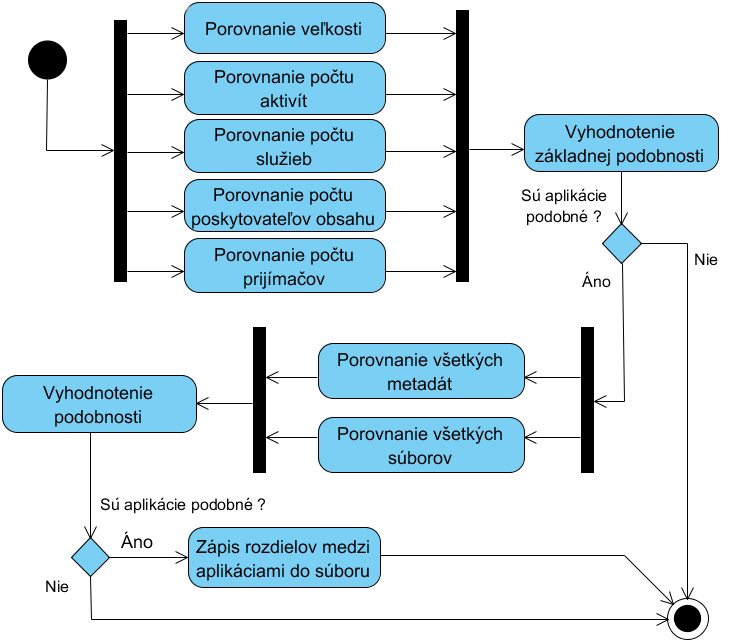
\includegraphics[height=10cm]{images/diagram.jpg}
  \end{center}
  \caption{Postup párového porovnávania APK súborov}
  \label{fig:compareFlow}
\end{figure}
\subsection{Implementácia}

Funkcionalita porovnávania a detekcie modifikovaných APK balíčkov je implementovaná v~programe \zv{ApkAnalyzer}. Používateľ môže aplikáciu spúšťať a zadávať jej parametre pomocou príkazového riadku. Funkcionalita porovnávania APK súborov sa spúšťa pomocou parametra \zv{–compare}. Vstup pre porovnávanie APK súborov nie sú samotné APK balíčky, ale JSON súbory, ktoré sú vytvorené aplikáciou \zv{ApkAnalyzer} počas analýzy APK balíčkov a obsahujú metadata o~aplikáciách (viď kapitola \ref{analyza}). Samotné porovnávanie prebieha párovo, každá aplikácia je porovnávaná so všetkými ostatnými. Proces porovnávania je paralelizovaný a každé dostupné procesorové jadro porovnáva inú dvojicu aplikácií. 

Porovnávanie a vyhodnocovanie podobnosti je rozdelené do viacerých etáp. Najskôr sa porovnávajú základné informácie o~APK súboroch a príslušných aplikáciách. Toto porovnanie využíva základné metadáta o~aplikáciách a zahŕňa veľkosť APK súboru, počet komponent z~ktorých sa aplikácia skladá (aktivity, služby, poskytovatelia obsahu, prijímače), počet rôznych obrázkových súborov a počet súborov definujúcich vzhľad obrazoviek.

Všetky tieto hodnoty sú číselné. Je nutné aby implementácia ich porovnávania bola funkčná nezávisle na veľkosti týchto číselných hodnôt. Taktiež je nutné zabezpečiť komutatívnosť, ktorá zaručí, že nezáleží na poradí porovnávania aplikácií a teda pre funkciu porovnávania $func$ platí \[func(A,B) = func(B,A)\] Získané hodnoty sú porovnávané s~minimálnymi hodnotami potrebnými na to, aby boli aplikácie považované za podobné. Tieto hodnoty je možné meniť editáciou súboru \zv{similarity.properties} v~koreňovej zložke projektu \zv{ApkAnalyzer}.

V~prípade detekcie základnej podobnosti sa porovnajú všetky súbory v~APK balíčkoch. Podobne ako v~aplikácií vyvinutej v~rámci projektu \zv{FSquaDRA}, na porovnanie sú využité SHA1 hashe súborov uložené v~\zv{MANIFEST.MF}. Separátne sú porovnávané súbory \zv{classes.dex}, \zv{resources.arsc}. Ostatné súbory sú porovnávané v~rámci kategórií: obrázkové súbory, súbory definujúce vzhľad obrazoviek a všetky ostatné súbory. Z dôvodu jednoduchšej práce s výstupom porovnania je spočítaný aj agregovaný rozdiel všetkých súborov v~APK balíčku. 

Zhoda súborov medzi dvomi APK balíčkami je určená pomocou Jaccardovho koeficientu podobnosti~\cite{Phillips2013}. Nech $A$ sú súbory v~danej kategórií v~jednom APK balíčku, $B$ sú súbory v~danej kategórií v~druhom porovnávanom APK balíčku. \[Jaccard Index(A,B) = \frac{|A~\cap B|}{ |A~\cup B|}\] Aplikácie sú považované za podobné v~prípade, že hodnota koeficientu podobnosti pre každú z~kategórií súborov v APK balíčku prekračuje minimálnu hodnotu definovanú v~súbore \zv{similarity.properties}. Určenie podobnosti v~tejto fáze prebieha len na základe rovnakých súborov. Okrem súborov sa porovnajú aj všetky hodnoty metadát získaných analýzou APK súboru. Tieto hodnoty sú použité ako informácie v detailnom výstupe porovnania.

\paragraph{Typ podobnosti}\mbox{}\\
Zhoda certifikátov a zhoda verzií aplikácií je vypočítaná za účelom určenia typu podobnosti daných aplikácií. Pri zhode verzií a certifikátov rozlišuje tri hodnoty – rovnaké, rozdielne alebo neurčené. Hodnota neurčené je použitá v~prípade, že sa dáta nepodarilo získať. Zhoda certifikátov sa určuje na základe hashu certifikátu. Tento údaj je v~kontexte detekcie modifikovaných APK súborov veľmi dôležitý. V~prípade zhody certifikátov je zaručené, že APK súbory pochádzajú od rovnakého vydavateľa. Pokiaľ sú certifikáty rozdielne, pôvodca súborov je s~najväčšou pravdepodobnosťou rozdielny. Zhoda verzií aplikácií je využitá na detekciu rovnakých aplikácií v~rozdielnych verziách.
Kombinácia týchto hodnôt určuje 9 kategórií podobnosti APK súborov. Každá z~týchto kategórií napovedá a vzájomnom vzťahu danej dvojice Android aplikácií. Najväčšia pravdepodobnosť, že aplikácia je prebalená, je v~prípade rovnakých verzií a zároveň rozdielnych certifikátov. 

\paragraph{Výstup porovnania}\mbox{}\\
V~prípade, že porovnávaná dvojica APK súborov je vyhodnotená ako podobná, \zv{ApkAnalyzer} vytvorí výstupný súbor vo formáte JSON obsahujúci rozdiely medzi danými aplikáciami. Tento súbor obsahuje rozdiely určené na základe metadát a porovnania aplikácií. Slúži ako jednoduchá obdoba linuxového príkazu \zv{diff} implementovaná nad APK súbormi. Obsahuje informácie o~modifikovaných parametroch a komponentoch aplikácií a taktiež zoznam upravených, nových alebo odstránených súborov. Zjednodušený príklad vzorového výstupného súboru obsahuje ukážka 7.1.
\begin{lstlisting} [language=json, caption= {Zjednodušená ukážka výstupu párového porovnanie APK súborov} \label{json:compare}]
{
  "nameA": "SoundHound  v6.7.5 apakrchive.com.apk",
  "nameB": "SoundHound 8 v6.3.3.apk",
  "hashCompareResult": {
    ...
    "modifiedDrawableFiles": [
      "res/drawable-nodpi-v4/ic_action_help.xml",
      ...
    ],
    "additionalDrawableFilesA": [
      "res/drawable-hdpi-v4/com_facebook_button_like_icon_selected.png",
      ...
    ],
    "additionalDrawableFilesB": [
      "res/drawable-hdpi-v4/ic_timestamp_clock_10dp.png",
      ...
    ],
    ...
  },
  "metadataCompareResult": {
    "fileSizeDifference": {
      "count": -2899397,
      "percentage": 16.98035514829626890787039883434772491455078125
    },
    "packageName": {
      "isSame": true
    },
    "versionCode": {
      "isSame": false,
      "difference": {
        "valueA": "10675",
        "valueB": "10633"
      }
    },
    "additionalActivitiesInA": [
      "com.soundhound.android.appcommon.activity.SplashScreenActivity",
      ...
    ],
    ...
  }
}
\end{lstlisting}

\subsection{Výsledky}
Vyhľadávanie možných prebalených APK súborov pomocou navrhnutej metódy určilo v~našej databáze viacero podozrivých aplikácií. Porovnávanie všetkých aplikácií v~našej databáze znamenalo viac ako dva milióny vykonaných párových porovnaní. Celkový čas potrebný na výpočet dosiahol približne 40 hodín. Porovnanie bolo vykonané na výkonnom ale bežnom komoditnom harvéri\footnote{Procesor Intel Core i7-4900MQ @ 2.80GHz , 16GB RAM, SSD disk}. V~čase potrebnom na porovnanie nie je započítaný čas na analýzu APK súborov a vytvorenie JSON súborov obsahujúcich metadáta. Vzhľadom na objem zbieraných dát a dekompiláciu APK balíčku pomocou nástroja \zv{ApkTool} počas analýzy (viď kapitola \ref{analyza}), je celkový čas potrebný na určenie prebalených súborov vyšší ako v~prípade metódy \zv{FSquaDRA}, avšak výstup nášho porovnania obsahuje informácie o~rozdieloch medzi jednotlivými APK súbormi. Dvojica APK súborov je považovaná za nadmieru podobnú v~prípade splnenia konfigurovateľných ktirétií podobnosti. Tie boli počas porovnávania nastavené na minimálnu zhodu 50\,\%, respektíve hodnotu \zv{Jaccard indexu} 0,5. Veľké množstvo aplikácií bolo vyhodnotených ako podobné, lebo sa jednalo o~rovnaké aplikácie v~rozdielnych verziách. Takéto aplikácie je možné vyfiltrovať s~využitím kategórie podobnosti, ktorá je každej porovnávanej dvojici priradená. \zv{ApkAnalyzer} automaticky rozdelí výstupné súbory do podpriečinkov podľa typu podobnosti APK súborov. Bolo identifikovaných 161 dvojíc aplikácií, ktoré splňovali kritériá zhody, boli v~rovnakej verzii, ale boli podpísané rôznymi certifikátmi.
  




{\csname captions\languagename\endcsname %% Temporarily override
%% the BibLaTeX localization with the original babel definitions.
\makeatletter %% Use the correct localization of the quotations.
  \thesis@selectLocale{\thesis@locale}\makeatother
\printbibliography[heading=bibintoc]} %% Print the bibliography.


%\makeatletter\thesis@blocks@clear\makeatother
\phantomsection %% Print the index and insert it into the
\addcontentsline{toc}{chapter}{\indexname} %% table of contents.
\printindex

\appendix %% Start the appendices.
\chapter{An appendix}

\begin{table}[htb]
\centering
  \begin{tabular}{|l l r|}
    \hline
    \textbf{Kód} & \textbf{Jazyk} &  \textbf{\%} \\\hline\hline
    es & španielsky & 61,7 \\
    de & nemecký & 59,6 \\
    fr & francúzsky & 59,4 \\
    ru & ruský & 58,1 \\
    ja & japonský & 57,6 \\
    it & taliansky & 57,4 \\
	ko & korejský & 56,9 \\
	zh-rcn & čínsky (zjednodušený) & 55,6\\
	zh-rtw & čínsky (tradičný)& 54,0\\
	pt & portugalský & 52,6\\
    \hline
  \end{tabular}
  \caption{Lokalizácia aplikácií}
  \label{tab:language}
\end{table}

\begin{table}[htb]
\centering
  \begin{tabular}{|l r|}
    \hline
    \textbf{Názov} & \textbf{\%} \\\hline\hline
    android.hardware.camera & 18,1 \\
    android.hardware.touchscreen & 16,1 \\
    android.hardware.telephony & 14,8 \\
    android.hardware.camera.autofocus & 10,6 \\
    android.hardware.location.gps & 10,2 \\
    android.hardware.location & 8,8 \\
    android.hardware.wifi & 8,4 \\
    android.hardware.location.network & 7,0\\
    android.hardware.bluetooth & 6,6\\
    android.hardware.touchscreen.multitouch & 6,0\\
    \hline
  \end{tabular}
  \caption{Najpoužívanejšie vlastnosti}
  \label{tab:features}
\end{table}

\begin{table}[htb]
\centering
  \begin{tabular}{|c c|}
    \hline
    \textbf{Verzia Android SDK} & \textbf{\%} \\\hline\hline
    9 & 21,3 \\
    8 & 18,4 \\
    7 & 14,2 \\
    14 & 10,5 \\
    10 & 8,1 \\
    4 & 7,0 \\
    3 & 5,6 \\
    15 & 3,7 \\
    5 & 3,7 \\
    11 & 2,1\\
    \hline
  \end{tabular}
  \caption{Hodnoty najnižsej vyžadovanej verzie Android SDK}
  \label{tab:minSdk}
\end{table}

\begin{table}[htb]
\centering
  \begin{tabular}{|c c|}
    \hline
    \textbf{Verzia Android SDK} & \textbf{\%} \\\hline\hline
    19 & 25,6 \\
    17 & 11,8 \\
    21 & 11,7 \\
    15 & 6,8 \\
    14 & 6,3 \\
    22 & 6,0\\
    16 & 5,7 \\
    18 & 5,6 \\
    20 & 3,8 \\
    8 & 2,9\\
    \hline
  \end{tabular}
  \caption{Hodnoty cieľovej verzie Android SDK}
  \label{tab:targetSdk}
\end{table}

\begin{table}[htb]
\begin{tabular}{|l|p{6.3cm}|}
 \hline
    \textbf{Atribút}& \textbf{Popis} \\\hline\hline
fileName & Názov analyzovaného APK súboru\\
sourceOfFile & Zdroj súboru\\
fileSize & Veľkosť APK súboru v bajtoch\\
dexSize & Veľkosť súboru \zv{classes.dex} v bajtoch \\
arscSize & Veľkosť súboru \zv{arscSize.dex} v bajtoch \\
packageName & Hodnota atribútu \zv{package} v elemente \zv{manifest}\\
versionCode & Hodnota atribútu \zv{android:versionCode} v elemente \zv{manifest}\\
installLocation & Hodnota atribútu \zv{android:installLocation} v elemente \zv{manifest}\\
numberOfActivities & Počet aktivít definovaných aplikáciou\\
numberOfServices & Počet služieb definovaných aplikáciou\\
numberOfContentProviders & Počet poskytovateľov obsahu definovaných aplikáciou  \\
numberOfBroadcastReceivers & Počet komponent typu \zv{BroadcastReceiver} definovaných aplikáciou\\
namesOfActivities & Názvy aktivít definovaných aplikáciou\\
namesOfServices & Názvy služieb definovaných aplikáciou\\
namesOfContentProviders & Názvy poskytovateľov obsahu definovaných aplikáciou\\
namesOfBroadcastReceivers & Názvy komponent typu \zv{BroadcastReceiver} definovaných aplikáciou\\
usesPermissions & Názvy povolení využívaných aplikáciou\\\hline
\end{tabular}
\end{table}
\begin{table}[htb]
\begin{tabular}{|l|p{6.5cm}|}
 \hline
    \textbf{Atribút}& \textbf{Popis} \\\hline\hline
usesLibrary & Názvy knižníc využívaných aplikáciou\\
permissions & Názvy povolení definovaných aplikáciou\\
permissionsProtectionLevel & Level ochrany povolení definovaných aplikáciou\\
usesFeature & Názvy vlastností využívaných aplikáciou\\
usesMinSdkVersion & Hodnota atibútu \zv{android:minSdkVersion} elementu \zv{uses-sdk}\\
usesTargetSdkVersion & Hodnota atribútu \zv{android:targetSdkVersion} elementu \zv{uses-sdk}\\
usesMaxSdkVersion & Hodnota atribútu \zv{android:maxSdkVersion} elementu \zv{uses-sdk}\\
supportsScreensResizeable & Hodnota atribútu \zv{android:resizeable} elementu \zv{supports-screens}\\
supportsScreensSmall & Hodnota atribútu \zv{android:smallScreens} elementu \zv{supports-screens}\\
supportsScreensNormal & Hodnota atribútu \zv{android:normalScreens} elementu \zv{supports-screens}\\
supportsScreensLarge & Hodnota atribútu \zv{android:largeScreens} elementu \zv{supports-screens}\\
supportsScreensXlarge & Hodnota atribútu \zv{android:xlargeScreens} elementu \zv{supports-screens}\\
supportsScreensAnyDensity & Hodnota atribútu \zv{android:anyDensity} elementu \zv{supports-screens}\\\hline
\end{tabular}
\end{table}
\begin{table}[htb]
\begin{tabular}{|l|p{7.2cm}|}
 \hline
    \textbf{Atribút}& \textbf{Popis} \\\hline\hline
fileName & Názov súboru s certifikátom\\
signAlgorithm & Algoritmus použitý na podpis\\
signAlgorithmOID & OID algoritmu použitého na podpis\\
startDate & začiatok platnosti certifikátu\\
endDate & koniec platnosti certifikátu\\
publicKeyMd5 & MD5 hash verejného klúča\\
certBase64Md5 & Base64 MD5 hash certifikátu\\
certMd5 & MD5 hash certifikátu\\
version & Verzia cetifikátu\\
issuerName & Názov vydávateľa vo formáte definovanom RFC 2253\\
subjectName & Názov subjektu vo formáte definovanom RFC 2253\\
locale & Lokalizácie súboru \zv{string.xml}\\
numberOfStringResource & Počet záznamov v súbore \zv{string.xml}\\
pngDrawables & Počet PNG obrázkov\\
ninePatchDrawables & Počet 9.PNG obrázkov\\
jpgDrawables &Počet JPG obrázkov\\
gifDrawables & Počet GIF obrázkov\\
xmlDrawablesr & Počet XML obrázkov\\
ldpiDrawables & Počet obrázkov v ldpi priečinku\\
mdpiDrawables & Počet obrázkov v mdpi priečinku\\
hdpiDrawables & Počet obrázkov v hdpi priečinku\\
xhdpiDrawables & Počet obrázkov v xhdpi priečinku\\
xxhdpiDrawables & Počet obrázkov v xxhdpi priečinku\\
xxxhdpiDrawablesr & Počet obrázkov v xxxhdpi priečinku\\
tvdpiDrawables & Počet obrázkov v tvdpi priečinku\\
nodpiDrawables & Počet obrázkov v nodpi priečinku\\\hline
\end{tabular}
\end{table}
\begin{table}[htb]
\begin{tabular}{|l|p{6.9cm}|}
 \hline
    \textbf{Atribút}& \textbf{Popis} \\\hline\hline
unspecifiedDpiDrawables & Počet obrázkov nezaradených v *dpi priečinku\\
rawResources & Počet súborov v \cesta{raw/} priečinku\\
layouts & Počet súborov v \cesta{res/layout*} priečinkoch\\
differentLayouts & Počet rôznych súborov v \cesta{res/layout*} priečinkoch\\
menu & Počet súborov v \cesta{res/menu} priečinku\\
dexHash & Hash súboru \zv{classes.dex} prevzatý zo súboru \zv{MANIFEST.MF}\\
arscHash & Hash súboru \zv{arscHash.dex} prevzatý zo súboru \zv{MANIFEST.MF}\\
drawableHash & Hashe a cesty k súborov z prečinku \cesta{res/drawable} prevzaté zo súboru \zv{MANIFEST.MF}\\
layoutHash & Hashe a cesty k súborov z prečinku \cesta{res/layout} prevzaté zo súboru \zv{MANIFEST.MF}\\
otherHash & Hashe a cesty k všetkým ostatným súborov v APK balíčku prevzaté zo súboru \zv{MANIFEST.MF}\\\hline
\end{tabular}
   
  \caption{Zbierané metadata o APK súbore}
  \label{tab:zbieraneData}
\end{table}




\end{document}
